\itemhead{p.113 练习 · 第1题（教材p.113）}{XJ-B1-C04-PR-P113-Y0217}
\label{XJ-B1-C04-PR-P113-Y0217}
{\footnotesize 湘教版教材p.113 / PDF第120页 / p.113 练习 / 第1题}
\field{原题}{在同一平面直角坐标系中画出 $y=5^x$ 和 $y=5^{-x}$ 的图象，并说明它们之间的关系。}
\field{参考答案}{$5^x$ 与 $5^{-x}$ 均过 $(0,1)$，前者递增后者递减，关于 $y$ 轴对称。取 $x=-1,0,1$ 时函数值分别为 $1/5,1,5$ 与 $5,1,1/5$。}
\begin{center}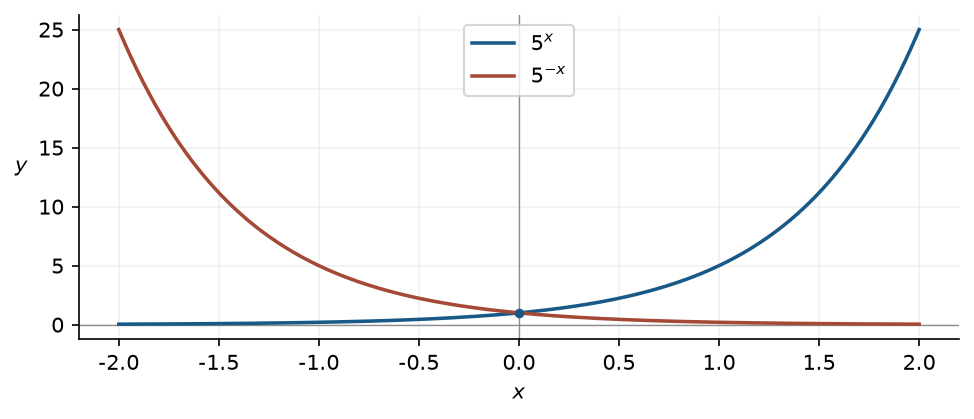
\includegraphics[width=.84\linewidth,height=.38\textheight,keepaspectratio]{figures/C04-PR113-1.png}\end{center}
\field{核对说明}{底数变化：答案册PDF31标p.112并作3\textasciicircum{}x图象；现教材p.113为5\textasciicircum{}x和5\textasciicircum{}(-x)，对称关系相同，作图点值必须更新。}
{\small \field{关联知识}{E01 指数函数的概念、图象与性质（教材帮p.150、151 / PDF159、160）；F09 图象平移、伸缩与对称（教材帮p.86、94 / PDF95、103）}
\field{方法与易错点}{先查底数条件，利用已知点定底数，再据单调性及图象求值或范围。 易错：只要求底数非负；漏排1；将 $a^x+b$ 当标准指数函数且仍用原值域。}
\field{答案依据}{答案册相关题组：PDF第31页（册内页30）；按当前题库原题逐项重算，不按旧版题号机械对套。}}
